\documentclass[uplatex,dvipdfmx,11pt,notheorems]{beamer}
%%%% 和文用 %%%%%
\usepackage{bxdpx-beamer}
\usepackage{pxjahyper}
% \usepackage{minijs}%和文用
\renewcommand{\kanjifamilydefault}{\gtdefault}%和文用

%%%% スライドの見た目 %%%%%
\usetheme{Madrid}
\setbeamertemplate{frametitle}[default][center]
\setbeamertemplate{navigation symbols}{}
\setbeamercovered{transparent}%好みに応じてどうぞ)
%\setbeamertemplate{footline}[page number]
%\setbeamerfont{footline}{size=\normalsize,series=\bfseries}
\setbeamercolor{footline}{fg=black,bg=black}
%\setbeamertemplate{footline}[frame number]
%%%%

%%%% 定義環境 %%%%%
\usepackage{amsmath,amssymb}
\usepackage{amsthm}
\theoremstyle{definition}
\newtheorem{theorem}{定理}
\newtheorem{definition}{定義}
\newtheorem{proposition}{命題}
\newtheorem{lemma}{補題}
\newtheorem{corollary}{系}
\newtheorem{conjecture}{予想}
\newtheorem*{remark}{Remark}
\renewcommand{\proofname}{}
%%%%%%%%%

%%%%% フォント基本設定 %%%%%
% \usepackage[T1]{fontenc}%8bit フォント
% \usepackage{textcomp}%欧文フォントの追加
% \usepackage[utf8]{inputenc}%文字コードをUTF-8
\usefonttheme{professionalfonts} %プロのフォント
\usepackage{color}
\usepackage{otf}%otfパッケージ
\usepackage{bm}%数式太字
%%%%%%%%%%
 
 \title[音場再現]{中間発表:重み付きモードマッチング法による音場再現}%[音場再現]{タイトル}
 \author[Ryosuke Horiuchi]{Ryosuke Horiuchi}%[音場再現]{名前}
 \institute[JPN]{Tokyo, Japan}%[略所属]{所属}
 \date{\today}%日付
 \begin{document}

 \begin{frame}[plain]\frametitle{}
 \titlepage %表紙
 \end{frame}

 \begin{frame}\frametitle{Contents}
 \tableofcontents %目次
 \end{frame}

 \section{問題設定}
 %\subsection{ガウス分布の確率密度関数}
 \begin{frame}\frametitle{問題設定}
 以下の図のようにある音場を、$\boldsymbol{r}_{l}(l \in\{1, \cdots, L\})$に置かれた$L$個の音源を用いて再現する.

    \begin{figure}[tb]
	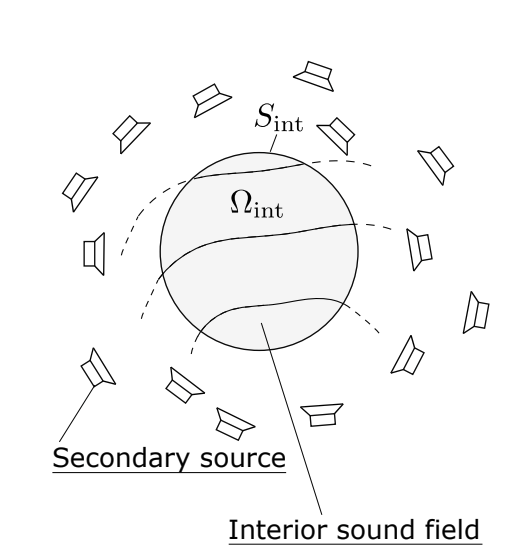
\includegraphics[width=4cm,clip]{intersimu0.png}
	\caption{想定する状況}
	\end{figure}
 \end{frame}

  \begin{frame}\frametitle{問題設定}
 $l$個目の音源の駆動信号を$d_{l}(\omega)$とし、ある場所$\boldsymbol{r}$への周波数$\omega$の伝達関数を$G\left(\boldsymbol{r} | \boldsymbol{r}_{l}, \omega\right)$とすると、$\boldsymbol{r}$における音圧は、
 $$p_{\text { syn }}(\boldsymbol{r}, \omega)=\sum_{l=1}^{L}  G\left(\boldsymbol{r} | \boldsymbol{r}_{l}, \omega\right)d_{l}(\omega)=\boldsymbol{g}(\boldsymbol{r}, \omega)^{\top} \boldsymbol{d}(\omega)$$
 とかける.
 ただし、$$\boldsymbol{d}(\omega)=\left[d_{1}(\omega), \cdots, d_{L}(\omega)\right]^{\top}$$
 $$\boldsymbol{g}(\boldsymbol{r}, \omega)=\left[G\left(\boldsymbol{r} | \boldsymbol{r}_{1}, \omega\right), \cdots, G\left(\boldsymbol{r} | \boldsymbol{r}_{L}, \omega\right)\right]^{\top}$$
 とした.\\
 注)以下は周波数を固定した議論であるので、$\omega$は省略する.
 \end{frame}

 \begin{frame}\frametitle{問題設定}
 再現したい領域を$V_{q}(q \in \{1, \cdots, Q\} )$とすると、その領域での二乗誤差の和は、
 $$\mathcal{J}=\sum_{q=1}^{Q} \int_{\boldsymbol{r} \in V_{q}}\left|p_{\text { syn }}(\boldsymbol{r})-p_{\mathrm{des}}(\boldsymbol{r})\right|^{2} \mathrm{d} \boldsymbol{r}=\sum_{q=1}^{Q} \int_{\boldsymbol{r} \in V_{q}}\left|\boldsymbol{g}(\boldsymbol{r})^{\top} \boldsymbol{d}-p_{\mathrm{des}}(\boldsymbol{r})\right|^{2} \mathrm{d} \boldsymbol{r}$$
と表され、この最小に基づき駆動信号$\mathrm{d}$を求める.\\
\vspace{10mm}
 \textcolor{red}{しかし、積分を解析的に解くことができない.}\\
 \vspace{10mm}
 注)簡単のため、以下では、$V_{q}(q \in \{1, \cdots, Q\} )$は球であるとする.
 \end{frame}

\section{球面調和関数を基底に用いる手法}


 \begin{frame}\frametitle{球面調和関数を基底に用いる手法}
 球面の内部で定義される任意の入射音場$p(\boldsymbol{r})$は、基底$\varphi_{\nu, \mu}(\boldsymbol{r})= j_{\nu}(k r) Y_{\nu, \mu}(\hat{\boldsymbol{r}})$を用いて、
 $$p(\boldsymbol{r})=\sum_{\nu,\mu} \alpha_{\nu,\mu} \varphi_{\nu, \mu}(\boldsymbol{r})$$
と展開できる.ただし、\\
\begin{itemize}
\item $k (= \omega/c)$:波数
\item  $j_{\nu}(\cdot)$:$\nu$次の第一種球面ベッセル関数
\item $Y_{\nu, \mu}(\cdot)$:球面調和関数
 \end{itemize}
例えば、点音源からの伝達関数は、以下のように球面調和関数展開できる.
$$\begin{aligned} G\left(\boldsymbol{r} | \boldsymbol{r}_{s}\right) &=\frac{\mathrm{e}^{\mathrm{i} k\left|r-r_{s}\right|}}{4 \pi\left|\boldsymbol{r}-\boldsymbol{r}_{s}\right|} \\ &=\mathrm{i} k \sum_{\nu=0}^{\infty} j_{\nu}(k r) h_{\nu}\left(k r_{s}\right) \sum_{\mu=-\nu}^{\nu} Y_{\nu,\mu}(\theta, \phi) Y_{\nu,\mu}\left(\theta_{s}, \phi_{s}\right)^{*} \end{aligned}$$

 \end{frame}

  \begin{frame}\frametitle{球面調和関数を基底に用いる手法}
 これを用いると、球面領域$V_{q}$の中心を、展開の中心として、
 $$\begin{array}{l}{G\left(\boldsymbol{r} | \boldsymbol{r}_{l}\right)=\sum_{\mu,\nu} c_{\mu, \nu,l}^{(q)} \varphi_{\mu,\nu}^{(q)}(\boldsymbol{r})} \\ {p_{\mathrm{des}}(\boldsymbol{r})=\sum_{\mu,\nu} b_{\mu,\nu}^{(q)} \varphi_{\mu,\nu}^{(q)}(\boldsymbol{r})}\end{array}$$
と基底変換をすることができる.
 \end{frame}

  \begin{frame}\frametitle{球面調和関数を基底に用いる手法}
ここで無限和を有限和で近似するために、$0 \leq \nu \leq M_{\nu}$で打ち切ると、$|\mu|\leq\nu$なので、全体は有限和となって、
$$\begin{array}{l}{G\left(\boldsymbol{r} | \boldsymbol{r}_{l}\right)=\sum_{\mu,\nu} c_{\mu, \nu,l}^{(q)} \varphi_{\mu,\nu}^{(q)}(\boldsymbol{r})} \approx \varphi^{(q)}(\boldsymbol{r})^{\top} \boldsymbol{C}_{l}^{(q)}\\ {p_{\mathrm{des}}(\boldsymbol{r})=\sum_{\mu,\nu} b_{\mu,\nu}^{(q)} \varphi_{\mu,\nu}^{(q)}(\boldsymbol{r})} \approx \varphi^{(q)}(\boldsymbol{r})^{\top} \boldsymbol{b}^{(q)}\end{array}$$
さらに、
$$\boldsymbol{g}(\boldsymbol{r}, \omega)^{\top}=\left[G\left(\boldsymbol{r} | \boldsymbol{r}_{1}, \omega\right), \cdots, G\left(\boldsymbol{r} | \boldsymbol{r}_{L}, \omega\right)\right] \approx \varphi^{(q)}(\boldsymbol{r})^{\top} \boldsymbol{C}^{(q)}$$
とかける.
ただし、$\varphi^{(q)}(\boldsymbol{r}) \in \mathbb{C}^{(M_{\nu}+1)^{2}}, \boldsymbol{C}^{(q)} \in \mathbb{C}^{\left(M_{\nu}+1\right)^{2} \times L}, \boldsymbol{b}^{(q)}(\boldsymbol{r}) \in \mathbb{C}^{(M_{\nu}+1)^{2}}$
$$\boldsymbol{C}^{(q)}  = \left[\boldsymbol{C}_{1}^{(q)}, \cdots,\boldsymbol{C}_{L}^{(q)} \right]$$

 \end{frame}

 

  \begin{frame}\frametitle{球面調和関数を基底に用いる手法}
これより、
	\begin{scriptsize}
	\begin{eqnarray}
	\mathcal{J} &\approx& \sum_{q=1}^{Q} \int_{r \in V_{q}}\left|\varphi^{(q)}(\boldsymbol{r})^{\top}\left(\boldsymbol{C}^{(q)} \boldsymbol{d}-\boldsymbol{b}^{(q)}\right)\right|^{2} \mathrm{d} \boldsymbol{r}\\
	&=&  \sum_{q=1}^{Q}\left\{\left(\boldsymbol{C}^{(q)} \boldsymbol{d}-\boldsymbol{b}^{(q)}\right)^{\mathrm{H}}\right.  \int_{\boldsymbol{r} \in V_{q}} \varphi^{(q)}(\boldsymbol{r})^{*} \varphi^{(q)}(\boldsymbol{r})^{\top} \mathrm{d} \boldsymbol{r}\left(\boldsymbol{C}^{(q)} \boldsymbol{d}-\boldsymbol{b}^{(q)}\right) \}\\
    &=& \sum_{q=1}^{Q}\left(\boldsymbol{C}^{(q)} \boldsymbol{d}-\boldsymbol{b}^{(q)}\right)^{\mathrm{H}} \boldsymbol{W}^{(q)}\left(\boldsymbol{C}^{(q)} \boldsymbol{d}-\boldsymbol{b}^{(q)}\right)
    \end{eqnarray}
	\end{scriptsize}
    ただし、$\boldsymbol{W}^{(q)} \in \mathbb{C}^{\left(2 M_{\nu}+1\right)^{2} \times\left(2 M_{\nu}+1\right)^{2}}$であり、$V_{q}$の半径を$ R_{\mathrm{int}}$として、
    $$w_{\nu_{1}, \mu_{1}}^{\nu_{2}, \mu_{2}}=\delta_{\nu_{1}, \nu_{2}} \delta_{\mu_{1}, \mu_{2}} w_{\mathrm{uni}, \nu_{1}}$$
    $$w_{\mathrm{uni}, \nu}=2 \pi R_{\mathrm{int}}^{3}\left(j_{\nu}\left(k R_{\mathrm{int}}\right)^{2}-j_{\nu-1}\left(k R_{\mathrm{int}}\right) j_{\nu+1}\left(k R_{\mathrm{int}}\right)\right)$$
    つまり、$\boldsymbol{W}^{(q)}$は対角行列となる.
 \end{frame}

  \begin{frame}\frametitle{球面調和関数を基底に用いる手法}
これより、
 よって、$\mathcal{J}$を$ \boldsymbol{d}$で偏微分することで、
$$\hat{\boldsymbol{d}}=\left(\sum_{q=1}^{Q} \boldsymbol{C}^{(q)^{\mathrm{H}}} \boldsymbol{W}^{(q)} \boldsymbol{C}^{(q)}+\lambda \boldsymbol{I}\right)^{-1} \sum_{q=1}^{Q} \boldsymbol{C}^{(q)^{\mathrm{H}}} \boldsymbol{W}^{(q)} \boldsymbol{b}^{(q)}$$
が得られる.\\
ただし、
$$\mathcal{J}=\sum_{q=1}^{Q} \int_{\boldsymbol{r} \in V_{q}}\left|p_{\mathrm{syn}}(\boldsymbol{r})-p_{\mathrm{des}}(\boldsymbol{r})\right|^{2} \mathrm{d} \boldsymbol{r} + \lambda  \boldsymbol{d}^{\mathrm{H}}  \boldsymbol{d}$$
と、ランク落ちを防ぐために$\lambda  \boldsymbol{d}^{\mathrm{H}} \boldsymbol{d}$を付け加えた.
 \end{frame}



\section{シミュレーション結果}
\begin{frame}\frametitle{シミュレーション結果}
スピーカを$12$個配置したと想定上で、周波数が$150$Hzの時.\\
再現領域:青い球内($Q=1$), 仮想点音源:青点
    \begin{figure}[tb]
	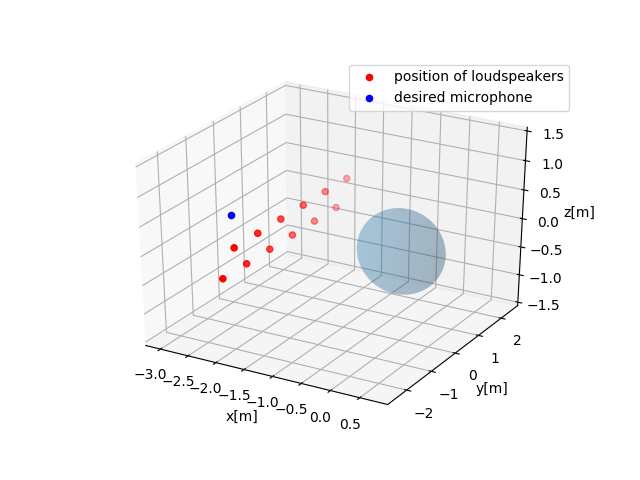
\includegraphics[width=8cm,clip]{intersimu4.png}
	\caption{シミュレーションの条件}
	\end{figure}

 \end{frame}
 \begin{frame}\frametitle{シミュレーション結果}
    \begin{figure}[tb]
	\centering
	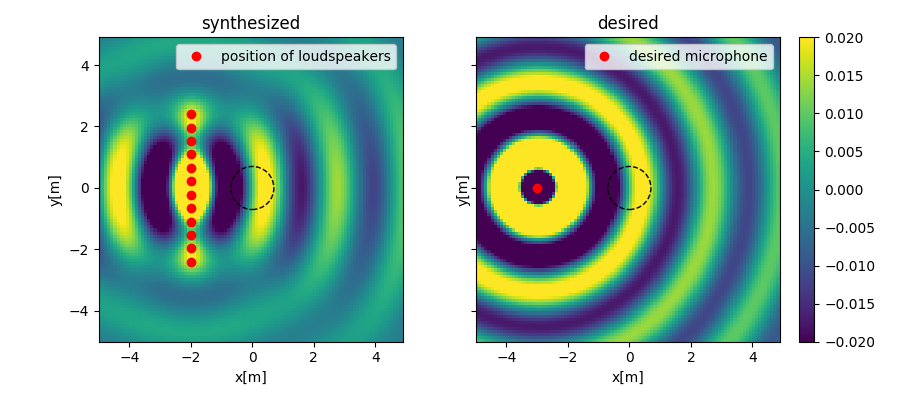
\includegraphics[width=8cm,clip]{intersimu1.png}
	\end{figure}
    \begin{figure}[tb]
	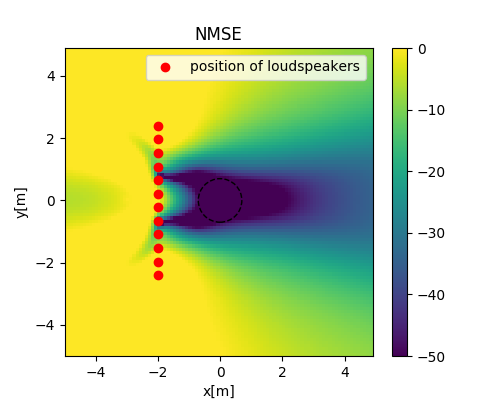
\includegraphics[width=3.5cm,clip]{intersimu2.png}
	\caption{左上:合成波、右上:目標波、下:$z=0$での正規化二乗誤差(単位:dB)}
	\end{figure}
 \end{frame}

\begin{frame}\frametitle{シミュレーション結果}
最大周波数を 4000 とし、幅 7.81( つまり、 512 分割)の周波数でそれぞれ
伝達関数を求め、逆フーリエ変換によって、時間領域でのフィルターを
求めた .
    \begin{figure}[tb]
	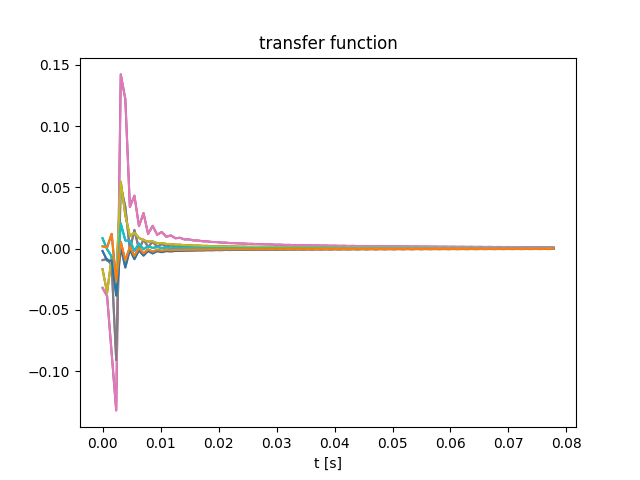
\includegraphics[width=8cm,clip]{intersimu3.png}
	\caption{時間領域でのフィルタ}
	\end{figure}
 \end{frame}



\section{今後の方針}
 \begin{frame}\frametitle{今後の方針}
 \begin{itemize}
    \item マルチゾーンの実装.
    \item 実環境で主観評価を行う.\\(時間的な制約があるので、被験者を集めるのは難しそう.)
    \item コードのリファクタリング.
\end{itemize}
 \end{frame}

 \section{参考文献}
 \begin{frame}\frametitle{参考文献}
    \begin{itemize}
        \item N. Ueno, S. Koyama, and H. Saruwatari,"Listening-area-informed sound field reproduction based on circular harmonic expansion"
        \item N. Ueno, S. Koyama, and H. Saruwatari,"Three-Dimensional Sound Field Reproduction Based on Weighted Mode-Matching Method"
        \item M. A. Poletti,"Three-Dimensional Surround Sound Systems Based on Spherical Harmonics"
    \end{itemize}
\end{frame}

 \begin{frame}\frametitle{Contents}
 \tableofcontents %目次
 \end{frame}
\end{document}
